\chapter{Modélisation UML et Conception Détaillée}

\section*{Introduction du chapitre}
La modélisation UML (\textit{Unified Modeling Language}) offre une représentation formelle et
normalisée de la structure et du comportement du système. Ce chapitre détaille la conception de
QuickTriage à travers trois familles de diagrammes complémentaires : le diagramme de cas
d'utilisation, qui décrit les interactions des acteurs avec le système ; le diagramme de
classes, qui en présente la structure statique ; et trois diagrammes de séquence, qui en
illustrent le comportement dynamique sur des scénarios représentatifs.

\section{Diagramme de cas d'utilisation}

\subsection{Présentation}
Le diagramme de cas d'utilisation (figure~\ref{fig:usecase}) recense les fonctionnalités
offertes par QuickTriage et les associe aux trois acteurs identifiés au chapitre~3 :
l'infirmier de tri, le médecin et l'administrateur.

\begin{figure}[h]
\centering
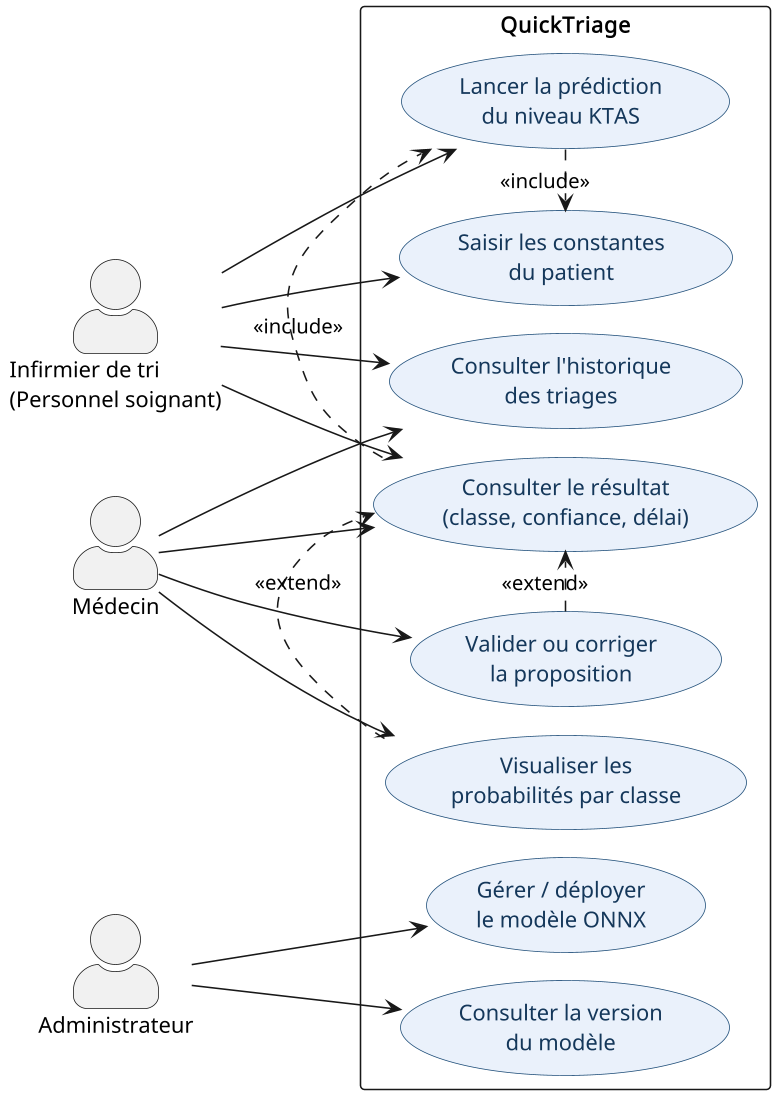
\includegraphics[width=0.95\textwidth]{images/usecase.png}
\caption{Diagramme de cas d'utilisation global de QuickTriage.}
\label{fig:usecase}
\end{figure}

\subsection{Analyse}
L'\textbf{infirmier de tri}, acteur principal, concentre le cœur du parcours opérationnel :
saisir les constantes, lancer la prédiction, consulter le résultat et accéder à l'historique.
Le \textbf{médecin} intervient en supervision : il consulte le résultat, visualise le détail
des probabilités et valide ou corrige la proposition du système. L'\textbf{administrateur}
prend en charge les tâches techniques : déploiement du modèle ONNX et consultation de sa
version.

Les relations entre cas d'utilisation précisent la logique fonctionnelle. La relation
\texttt{<<include>>} entre « Lancer la prédiction » et « Saisir les constantes » traduit le
fait que la prédiction présuppose nécessairement une saisie préalable ; de même, « Consulter le
résultat » inclut la prédiction. Les relations \texttt{<<extend>>} reliant « Visualiser les
probabilités » et « Valider ou corriger » à « Consulter le résultat » expriment des
comportements optionnels, déclenchés à la discrétion de l'utilisateur. Cette structuration
garantit que l'acte de triage reste rapide par défaut, tout en autorisant un approfondissement
sur demande.

\section{Diagramme de classes}

\subsection{Présentation}
Le diagramme de classes (figure~\ref{fig:classes}) décrit la structure statique de la solution,
en distinguant les composants du backend J2EE et les modèles du frontend Flutter.

\begin{figure}[h]
\centering
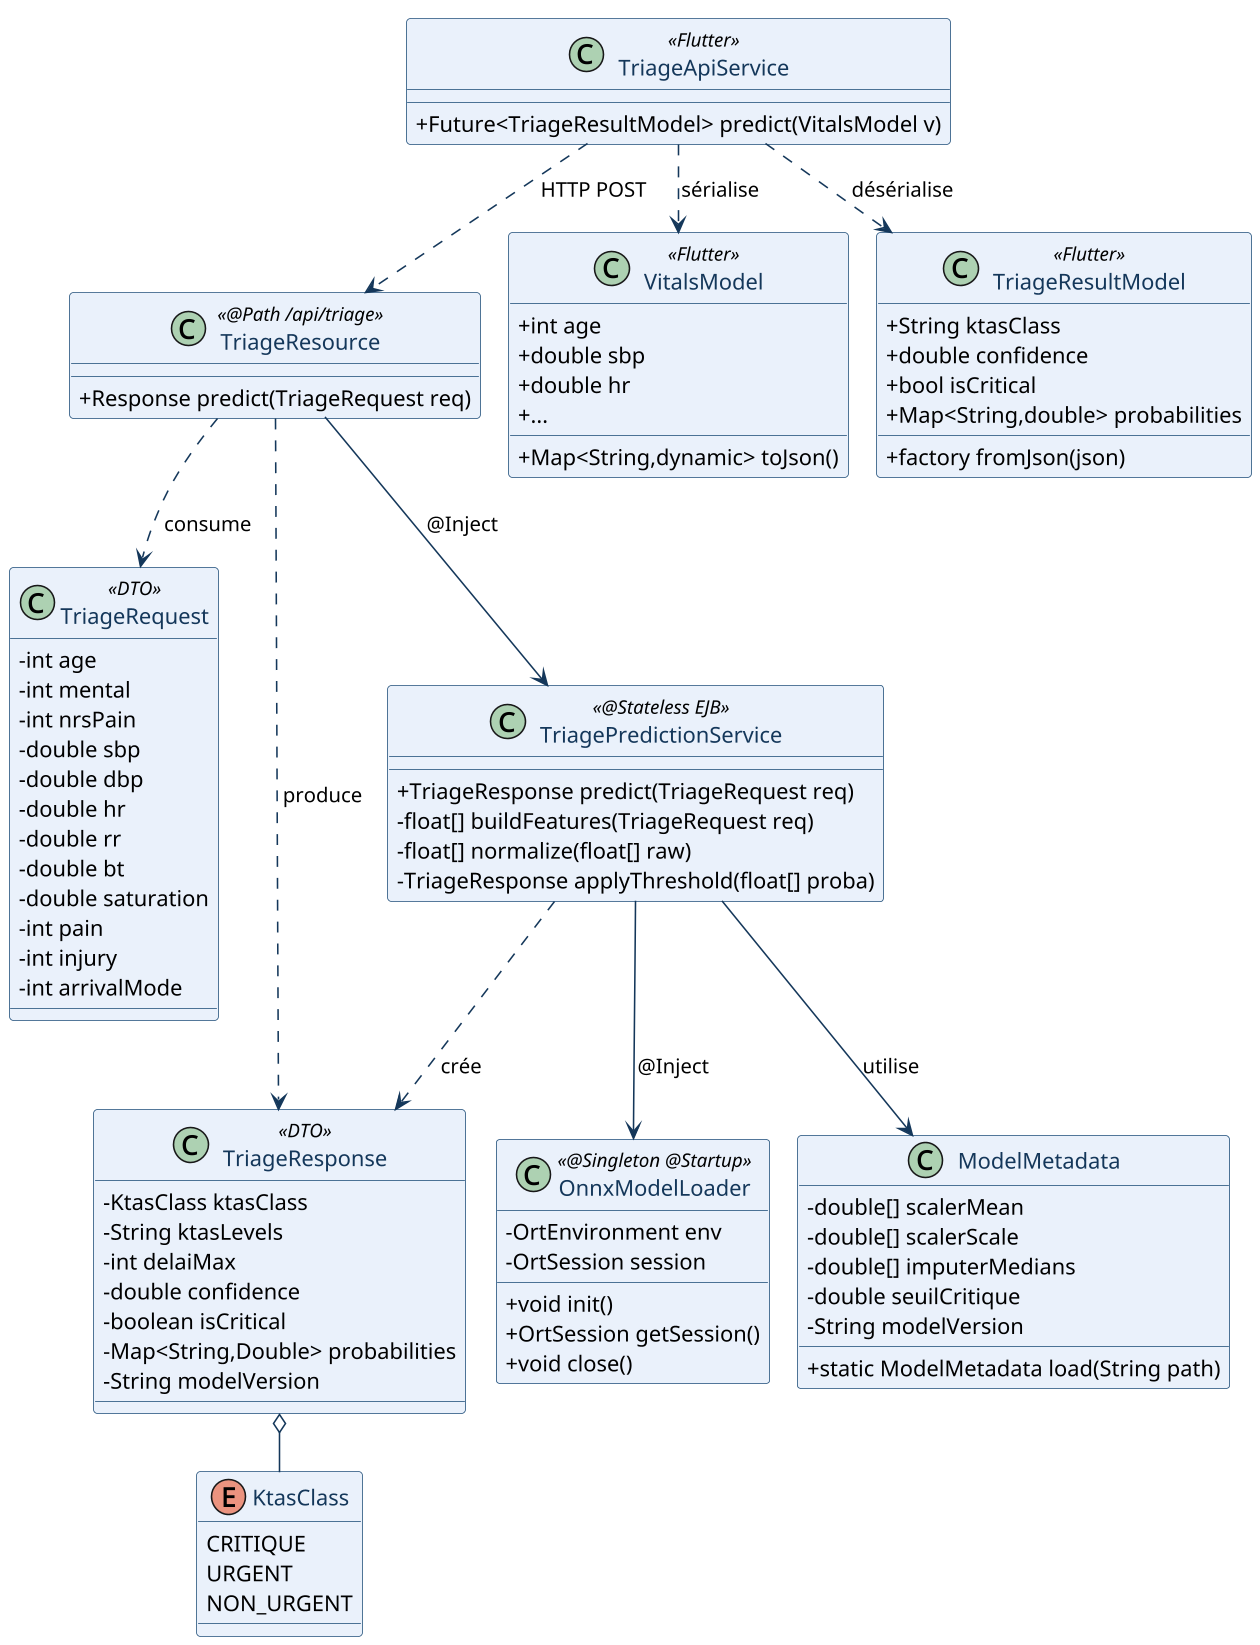
\includegraphics[width=\textwidth]{images/class.png}
\caption{Diagramme de classes de QuickTriage (backend J2EE et modèles frontend).}
\label{fig:classes}
\end{figure}

\subsection{Analyse des classes du backend}
Le backend s'organise autour de cinq classes et d'une énumération :
\begin{itemize}
  \item \texttt{TriageRequest} et \texttt{TriageResponse} sont des \textbf{DTO}
  (\textit{Data Transfer Objects}). Le premier transporte les constantes vitales saisies
  (âge, état mental, douleur, SBP, DBP, HR, RR, BT, saturation, etc.) ; le second véhicule le
  résultat (classe KTAS, délai maximal, confiance, indicateur \texttt{isCritical}, probabilités
  par classe et version du modèle).
  \item \texttt{TriageResource} est la ressource \textbf{JAX-RS} (\texttt{@Path /api/triage})
  qui consomme un \texttt{TriageRequest} et produit un \texttt{TriageResponse}. Elle délègue le
  traitement au service métier.
  \item \texttt{TriagePredictionService} est l'\textbf{EJB \texttt{@Stateless}} qui orchestre
  la prédiction : \texttt{buildFeatures()} construit le vecteur, \texttt{normalize()} applique
  la standardisation et \texttt{applyThreshold()} décide de la classe selon le seuil de
  criticité.
  \item \texttt{OnnxModelLoader} est le bean \textbf{\texttt{@Singleton @Startup}} qui détient
  l'\texttt{OrtEnvironment} et l'\texttt{OrtSession}, initialisés une fois au démarrage et
  exposés via \texttt{getSession()}.
  \item \texttt{ModelMetadata} encapsule les paramètres de prétraitement chargés depuis
  \texttt{metadata\_v3.json} (moyennes et écarts-types du scaler, médianes de l'imputeur, seuil
  de la classe \textsc{Critique}, version du modèle).
  \item L'énumération \texttt{KtasClass} matérialise les trois classes métier : \texttt{CRITIQUE},
  \texttt{URGENT} et \texttt{NON\_URGENT}.
\end{itemize}

Les associations traduisent les dépendances d'injection (\texttt{@Inject}) : la ressource
dépend du service, qui dépend lui-même du chargeur de modèle et exploite les métadonnées. Ce
graphe de dépendances reflète fidèlement la séparation des responsabilités décrite au
chapitre~4.

\subsection{Analyse des modèles du frontend}
Côté Flutter, trois classes assurent le miroir client : \texttt{VitalsModel} représente les
constantes saisies et fournit une méthode \texttt{toJson()} de sérialisation ;
\texttt{TriageResultModel} représente le résultat et propose une fabrique \texttt{fromJson()}
de désérialisation ; \texttt{TriageApiService} encapsule l'appel HTTP \texttt{POST} vers la
ressource REST, sérialisant la requête et désérialisant la réponse. Cette symétrie entre les
DTO du backend et les modèles du frontend garantit un contrat d'échange clair et maintenable.

\section{Diagrammes de séquence}
Les diagrammes de séquence décrivent les interactions temporelles entre les objets pour trois
scénarios représentatifs : le cycle complet d'une demande de triage, le détail de l'appel REST
et de l'inférence, et la validation clinique avec historisation.

\subsection{Scénario 1 : cycle complet d'une demande de triage}
Le premier scénario (figure~\ref{fig:seqtriage}) retrace le parcours nominal de bout en bout,
depuis la saisie des constantes par l'infirmier jusqu'à l'affichage du résultat coloré.

\begin{figure}[h]
\centering
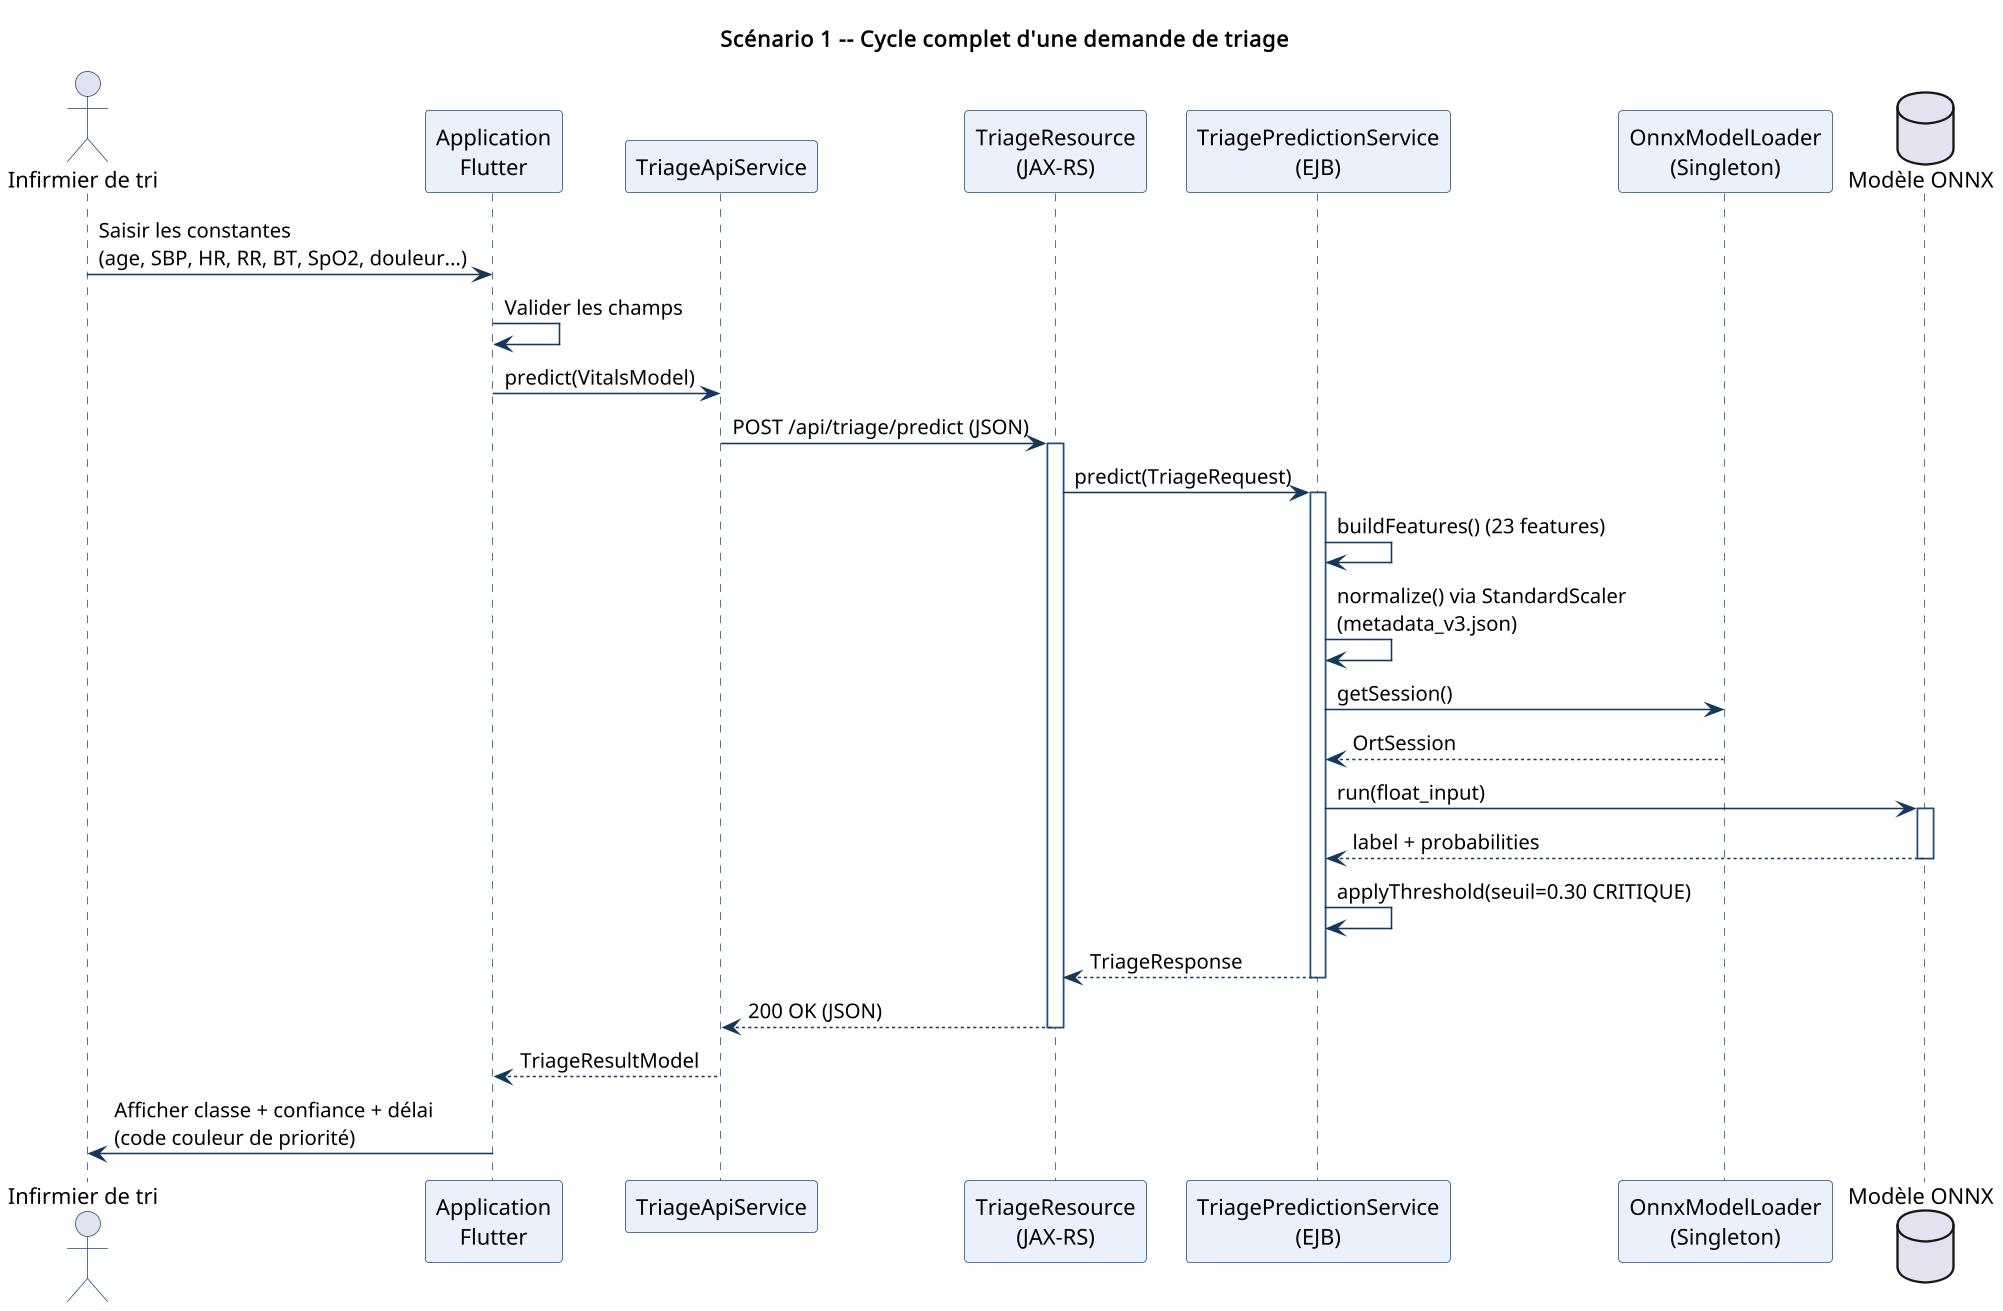
\includegraphics[width=\textwidth]{images/seq_triage.png}
\caption{Scénario 1 -- Cycle complet d'une demande de triage.}
\label{fig:seqtriage}
\end{figure}

\noindent Ce diagramme met en évidence la chaîne d'appels : l'application Flutter valide les
champs puis invoque \texttt{TriageApiService}, qui émet une requête \texttt{POST} vers
\texttt{TriageResource}. Le service métier construit et normalise les caractéristiques, sollicite
la session ONNX maintenue par \texttt{OnnxModelLoader}, applique le seuil de criticité (0,30 pour
la classe \textsc{Critique}) et retourne la réponse. Le résultat remonte jusqu'à l'interface, où
il est affiché avec le code couleur de priorité. On observe que le chargement du modèle n'apparaît
pas dans ce flux : il a eu lieu une fois pour toutes au démarrage du serveur.

\subsection{Scénario 2 : traitement de la requête REST et inférence ONNX}
Le deuxième scénario (figure~\ref{fig:seqrest}) zoome sur le traitement côté backend, en
détaillant les étapes de prétraitement et la logique de décision.

\begin{figure}[h]
\centering
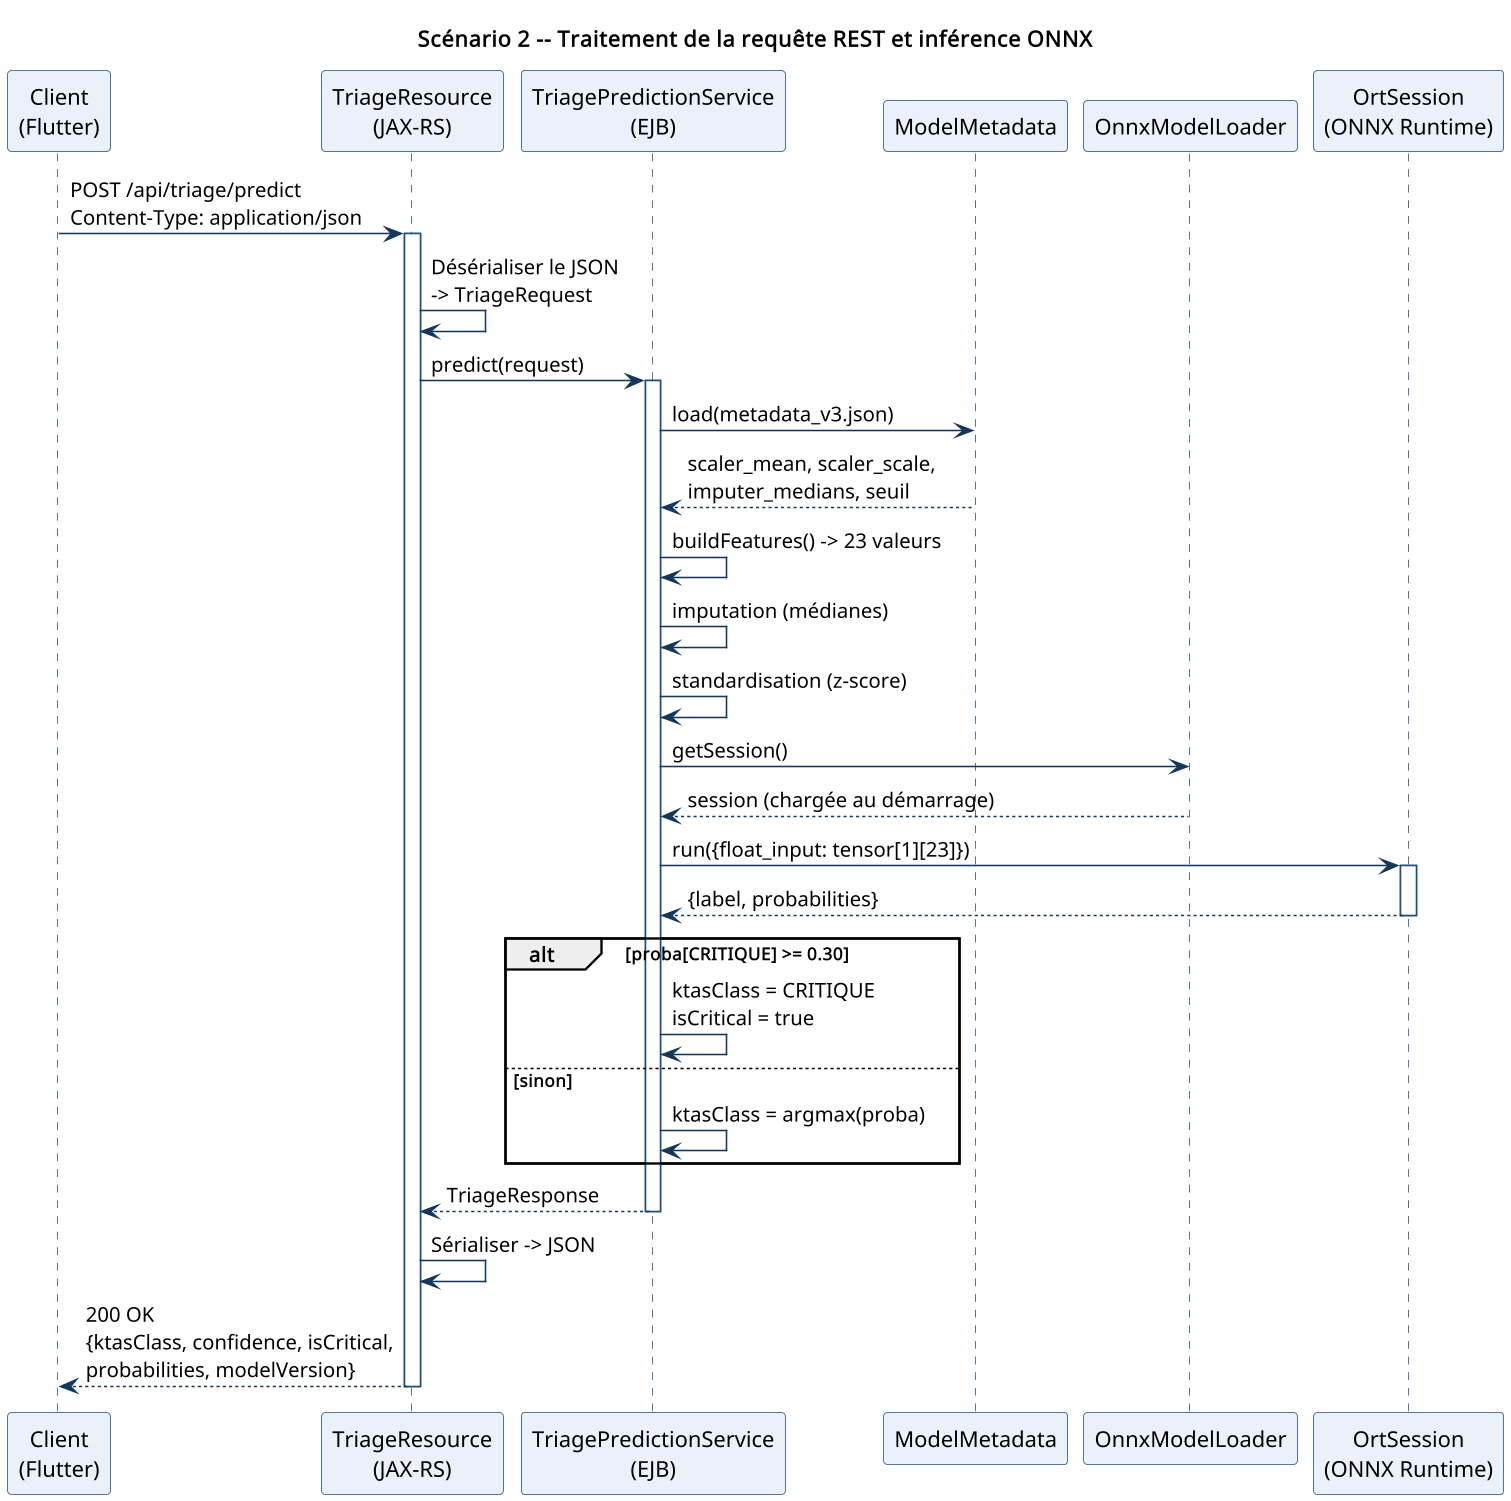
\includegraphics[width=\textwidth]{images/seq_rest.png}
\caption{Scénario 2 -- Traitement de la requête REST et inférence ONNX.}
\label{fig:seqrest}
\end{figure}

\noindent Après désérialisation du JSON en \texttt{TriageRequest}, le service charge les
métadonnées (\texttt{ModelMetadata}), construit les 23 caractéristiques, applique l'imputation par
médianes puis la standardisation z-score. Il récupère ensuite la session auprès du chargeur et
exécute l'inférence sur un tenseur de forme $[1][23]$. Le fragment \texttt{alt} formalise la
règle de décision orientée sécurité : si la probabilité de la classe \textsc{Critique} atteint le
seuil de 0,30, le patient est classé \textsc{Critique} et \texttt{isCritical} est positionné à
vrai ; sinon, la classe retenue est celle de probabilité maximale. La réponse JSON consolide
l'ensemble des informations (classe, confiance, probabilités, version du modèle).

\subsection{Scénario 3 : validation clinique et historisation}
Le troisième scénario (figure~\ref{fig:seqvalid}) illustre l'intervention du médecin, qui valide
ou corrige la proposition, ainsi que l'historisation de la décision finale.

\begin{figure}[h]
\centering
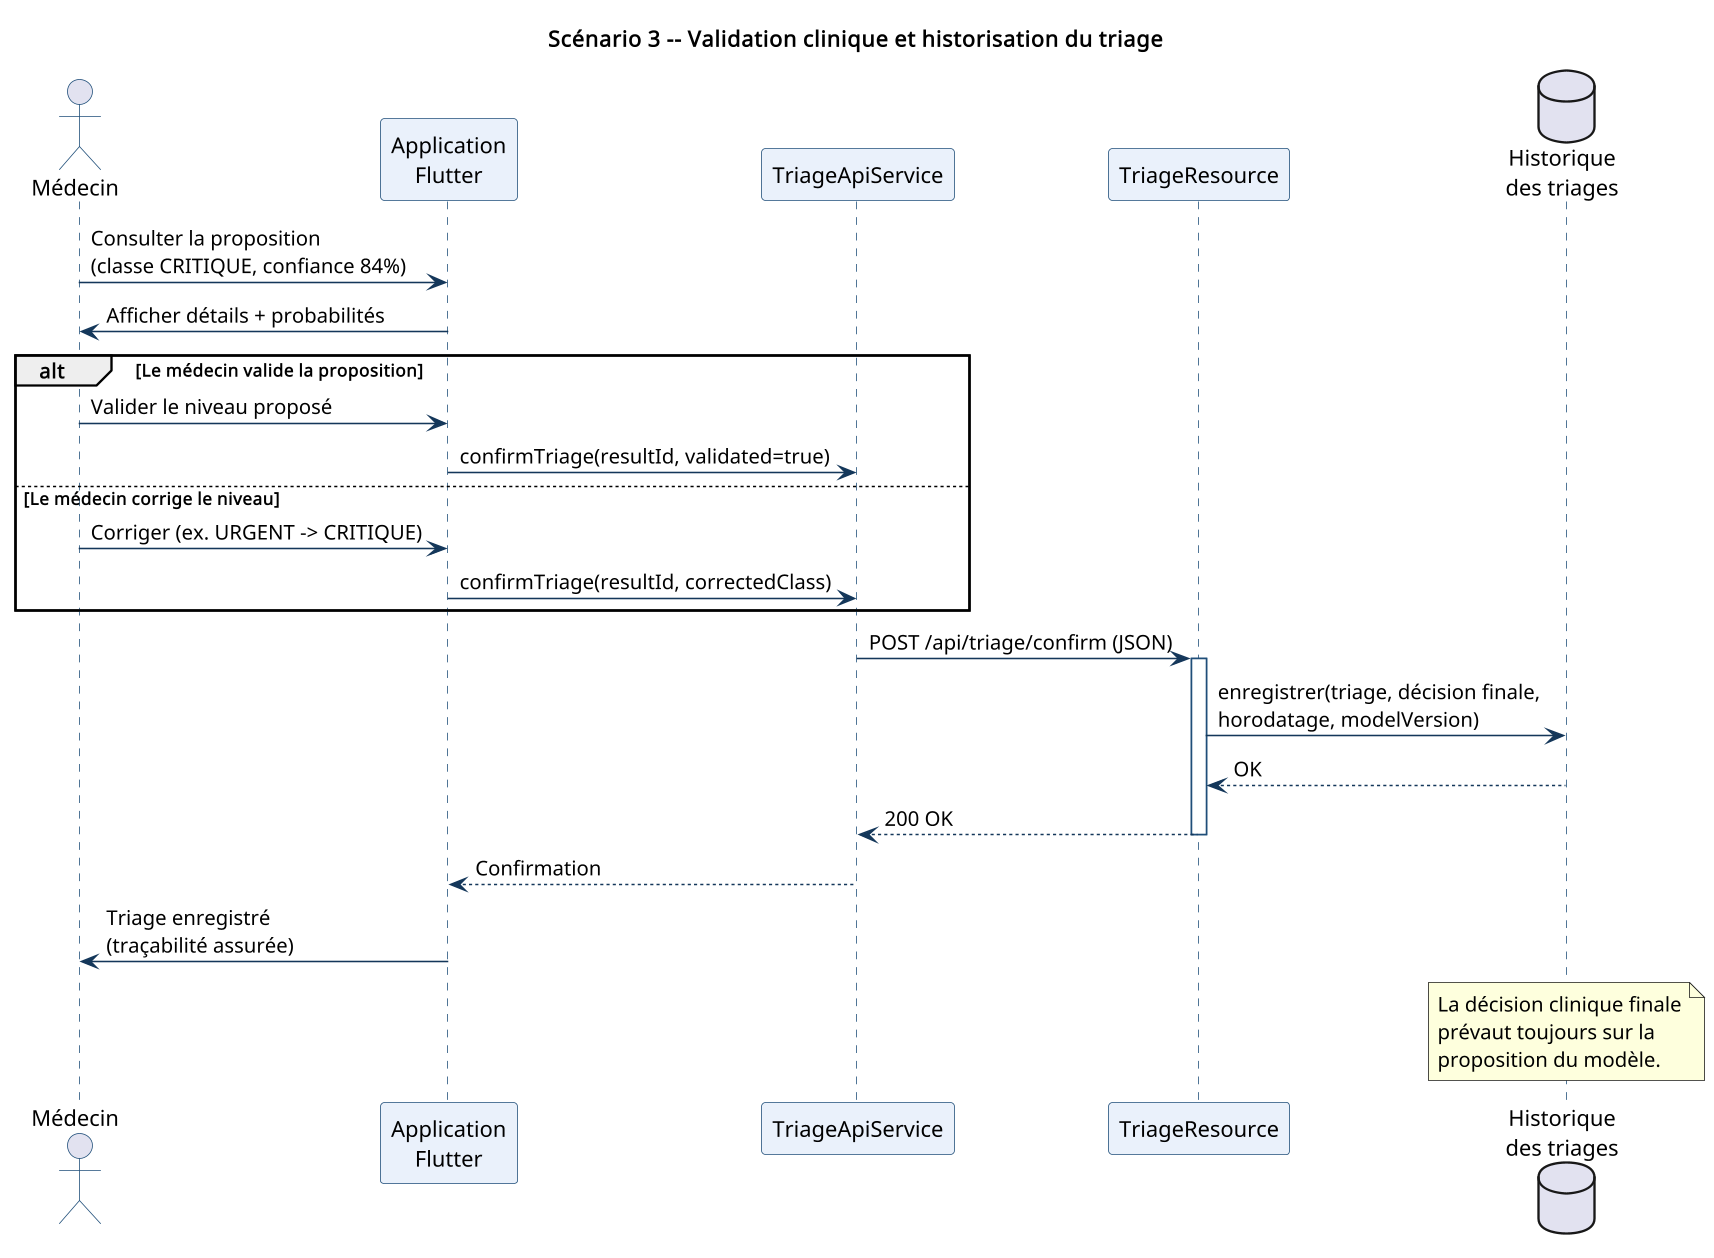
\includegraphics[width=\textwidth]{images/seq_validation.png}
\caption{Scénario 3 -- Validation clinique et historisation du triage.}
\label{fig:seqvalid}
\end{figure}

\noindent Le médecin consulte la proposition assortie des probabilités. Le fragment \texttt{alt}
distingue deux issues : la validation du niveau proposé ou sa correction (par exemple le passage
d'\textsc{Urgent} à \textsc{Critique}). Dans les deux cas, la décision est transmise via
\texttt{POST /api/triage/confirm} et enregistrée dans l'historique des triages avec son
horodatage et la version du modèle. La note finale du diagramme rappelle le principe cardinal de
QuickTriage : \textbf{la décision clinique finale prévaut toujours sur la proposition du modèle}.
Ce scénario matérialise ainsi l'exigence de traçabilité et le positionnement du système comme
simple aide à la décision.

\section*{Conclusion du chapitre}
Ce chapitre a formalisé la conception détaillée de QuickTriage au moyen de la modélisation UML :
le diagramme de cas d'utilisation a clarifié les interactions des acteurs, le diagramme de classes
a exposé la structure statique des couches backend et frontend, et les trois diagrammes de séquence
ont décrit le comportement dynamique du système sur des scénarios représentatifs. Ces modèles
établissent un pont rigoureux entre l'architecture du chapitre précédent et l'implémentation
concrète, objet du chapitre suivant.
